\section{Genetic Algorithms}

\subsection{History}

Genetic algorithms are optimisation techniques that employ the same rationale as classical Evolution as seen in nature.

Genetic Algorithms can trace their origins back to the late 1960s when they were first proposed by John Holland, though he then referred to them as \textit{Genetic Plans}\footnote{This distinction was made to emphasise the \textit{"centrality of computation in defining and implementing the plans"}\cite{hollandAdaptationNaturalArtificial1992a}}. Holland went on to write the first book on the subject titled \textit{Adaptation in Natural and Artificial Systems}\cite{hollandAdaptationNaturalArtificial1992a} in 1975. The field did not find much reception with Holland stating in the preface to the 1992 rerun:

\begin{displayquote}
\textit{``When this book was originally published I was very optimistic, envisioning extensive reviews and a kind of 'best seller' in the realm of monographs. Alas! That did not happen.``}
\end{displayquote}

However, in the early nineties, Genetic algorithms surged in popularity along with the area of Artificially Intelligent planning as a whole leading to Holland republishing his book and solidifying his position as the field's founder.

\subsection{Definition}
In a general sense, optimisation techniques work to find the set of parameters $\mathcal{P}$ that minimise an objective function $\mathcal{F}$. 
Genetic algorithms approach this by representing these sets as individuals in a population, $P$. Over the course of multiple generations, the best solutions are determined and promoted until termination criteria are met or the maximum number of generations is reached.

As our candidates are essentially a collection of parameters to the function we are trying to optimise, we can extend our metaphor further by mapping each element of a individual to a \textit{gene} in a individual's genome. 

The representation we use in a GA is problem specific. Often we have to provide functions to facilitate the mapping between the problem specific set of possible solutions and the encoded genotype space in which we optimise. The most basic representation being a string of binary numbers.

Genetic algorithms are both \textit{probabilistically optimal} and \textit{probabilistically complete}\cite{kalaOnroadIntelligentVehicles2016} meaning that: given infinite time, not only will the algorithm find \textit{a} solution, (if one exists), it will find \textbf{the} optimal solution from the set of all possible solutions, $\mathcal{P}^*$.

\begin{algorithm}[H]
	\label{alg:GenericGA}
	\SetAlgoLined
	\KwResult{Best Solution, $p_{ \texttt{best}}$}	
	Generate initial population, $P_0$ of size $n$\;
	Evaluate fitness of each individual in $P_0$, $\{F(p_{0,1},\ldots, p_{0,n})\}$\;
	\While{termination criteria are not met}{
		\textbf{Selection}: Select individuals from $P_t$ based on their fitness\;
		\textbf{Variation}: Apply variation operators to parents from $P_t$ to produce offspring\;
		\textbf{Evaluation}: Evaluate the fitness of the newly bred individuals\;
		\textbf{Reproduction}: Generate a new population $P_{t+1}$ using individuals from $P_t$ as well as the newly bred candidates.\;
		$t$++
	}
	return $p_{\texttt{best}}$

	\caption{Modern Generic Genetic Algorithm}
\end{algorithm}

\begin{figure}[htpb]
    \centering
    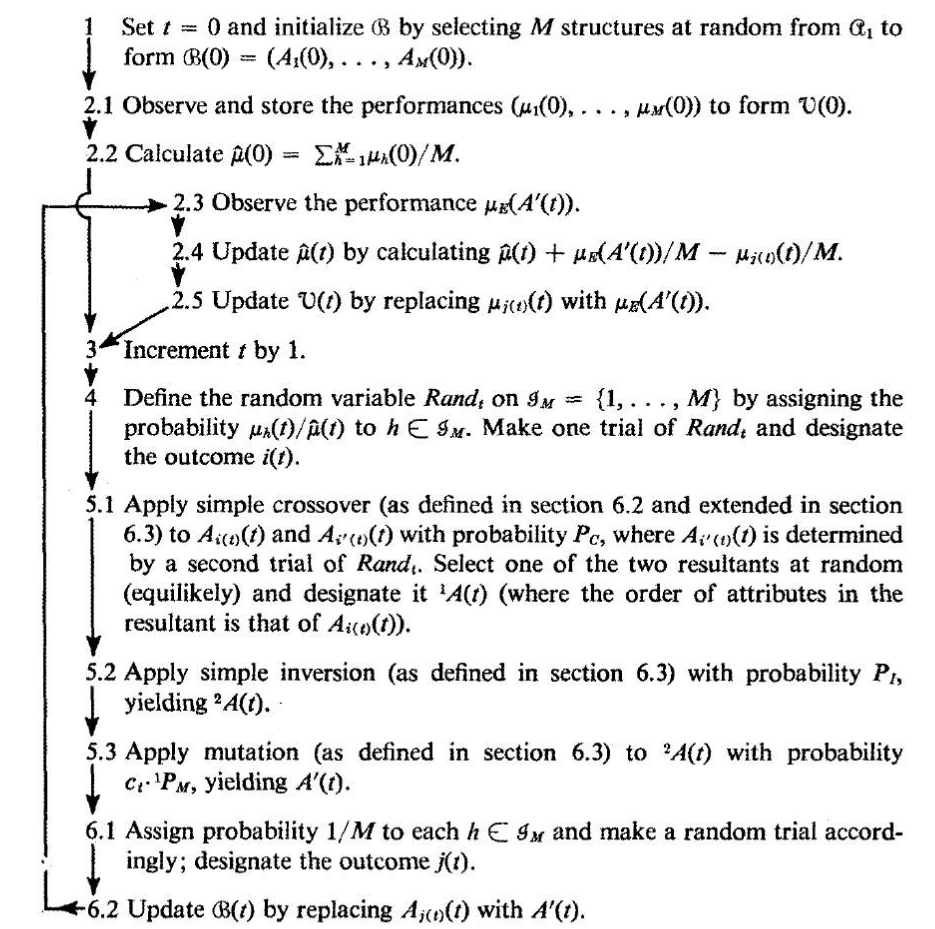
\includegraphics[width=\linewidth]{hollandAlg}
    \caption{GA algorithm outlined in Holland's Original Book\cite{hollandAdaptationNaturalArtificial1992a}}
    \label{fig:hollandAlg}
\end{figure}

As you can see from Figure \ref{fig:hollandAlg} and Algorithm \ref{alg:GenericGA} the overall shape of GAs has not changed substantially over the course of the past 50 years. Being comprised of a series of operations that a starting population is piped through until criteria are met.

\subsection{Selection}

The selection procedure is the process by which the next generation of individuals is created from the current population. Individuals are selected relative to their fitness as determined by the Objective (fitness) function $\mathcal{F}$. 

Some methods select only the best solutions by fitness. Others employ a more stochastic approach such as the Monte Carlo method\cite{metropolis1987beginning} to increase diversity and reduce complexity.

\subsection{Variation}

Variation in a GA is the process of altering the genome individuals to further explore the search space via stochastic local search.
We perform this using two distinct sub-operations: Mutation and Crossover.

\subsubsection{Mutation}

In mutation we alter each gene with a set probability $p_m$ known as the \textit{mutation rate}. A standard value for a mutation rate is $ \frac{1}{L} $ but it can fall anywhere in the range $p_m \in [ \frac{1}{L} , \frac{1}{2} ] $ where $L$ is the length of the genome.
In binary coded GAs we alter a given gene by \textit{flipping} it's value.
In real-coded GAs mutation operators include: 
\begin{itemize}
    \item Uniform Mutation
    \item Non-Uniform Mutation
    \item Gaussian Mutation 
\end{itemize}

A low value for $p_m$ a new individual which can be shown to be \textit{close} to it's parents in the search space relative to their \textit{Hamming distance}\footnote{Hamming Distance: The metric for comparing two binary data strings. The Hamming distance between two strings is the number of bit position in which they differ.} if using a Binary coded GA. In real-coded GAs they can be shown to be close by the Euclidean distance between them.

\subsubsection{Crossover}

Crossover is a binary operation, taking two randomly selected \textit{parents} from the population $P_t$ with a probability $p_c \in [0,1]$ 

There are two major forms of crossover for binary coded GAs: $n>1$ point crossover and Uniform crossover. 

For real-coded GAs you instead have a selection of Crossover operators including:

\begin{itemize}
    \item Flat crossover
    \item Simple crossover
    \item Whole arithmetic crossover
    \item Local arithmetic crossover
    \item Single arithmetic crossover
    \item BLX-$\alpha$ crossover
\end{itemize}

\subsection{Evaluation}
After developing potential new individuals, the fitness of these new individuals is calculated using the objective function, $\mathcal{F}$
\subsection{Reproduction}
Here the next generation of individuals is constructed. There are multiple potential methods employed here with the simplest being to just replace the lest fit individuals with additional copies of the fitter individuals, be they pre-existing or newly generated.

In this stage various heuristics or alternative strategies can be implemented to speed up or slow down the convergence rate. Whilst their fitness may be low, having a diverse population allows for more of the search space to be explored. If the algorithm converges too quickly it may get \textit{stuck} in local minima. 

\section{Autonomous Road Networks}

\section{Quantum Genetic Algorithms}

\section{Alternative Technologies}
